\documentclass[conference]{IEEEtran}
\usepackage{graphicx}
\usepackage{booktabs}
\usepackage{array}
\usepackage{url}
\usepackage{cite}
\usepackage{amsmath}
\usepackage{listings}
\usepackage{xcolor}

\lstset{
    basicstyle=\ttfamily\small,
    breaklines=true,
    keywordstyle=\color{blue},
    commentstyle=\color{gray},
    stringstyle=\color{red},
    backgroundcolor=\color{lightgray!20},
    frame=single,
    rulecolor=\color{black!30},
    stepnumber=1,
    numberstyle=\tiny,
    captionpos=b
}

\begin{document}

\title{AI Resume \& Job Match Analyzer\\
\large Short Project Report}

\author{\IEEEauthorblockN{Vaibhav Krishali}\\
\IEEEauthorblockA{Emerging Technologies Project\\
Date: April 2, 2026}}

\maketitle

\begin{abstract}
This project presents an AI-assisted Resume and Job Match Analyzer built using FastAPI and a lightweight web interface. The system evaluates resume quality, recommends suitable roles, and compares resume-job fit through ATS-style scoring. For ML Engineer roles specifically, it provides role-targeted skill gap analysis, actionable ATS suggestions, and rewritten bullet points emphasizing machine learning impact. A resume-upgrade module generates an improved version with before-vs-after comparison and produces an Overleaf-ready LaTeX draft with PDF preview support. The system is designed for accessibility, remaining functional without paid APIs by supporting local and heuristic analysis modes.
\end{abstract}

\section{Introduction}
\textbf{Problem Statement:} Many technical professionals, including ML engineers and data scientists, struggle to understand whether their resumes align with industry expectations and target job descriptions. Manual review processes are slow, inconsistent, and often miss ATS (Applicant Tracking System) keywords critical for job application success.

\textbf{Importance of Topic:} Modern hiring pipelines increasingly depend on ATS filtering before human review. For specialized roles like ML Engineer, the gap between candidate qualifications and job requirements can be subtle but significant. A structured, role-aware analyzer helps candidates identify specific skill gaps (e.g., missing TensorFlow/PyTorch mentions) and improve resume quality with quantified metrics and technical depth before submitting applications.

\textbf{Project Objective:} The project aims to build a practical web application that can (i) score CV readiness using role-agnostic heuristics, (ii) suggest relevant roles based on resume content, (iii) perform role-specific matching with targeted skill overlap analysis, and (iv) generate an upgraded resume draft with before-vs-after comparison highlighting improvements.

\section{Literature Review}
\begin{table}[htbp]
\caption{Literature Review Summary}
\label{tab:lit_review}
\centering
\footnotesize
\begin{tabular}{p{0.18\linewidth} p{0.17\linewidth} p{0.28\linewidth} p{0.27\linewidth}}
\toprule
\textbf{Work} & \textbf{Year} & \textbf{Key Contribution} & \textbf{Gap Addressed in This Project} \\
\midrule
OpenAI API Documentation~\cite{openai_docs} & 2025 & Structured LLM output for text analysis tasks. & Added fallback chain (OpenAI/Groq/local/heuristic) for reliability and cost control. \\
Groq API Documentation~\cite{groq_docs} & 2025 & Fast inference for LLM-based JSON generation. & Integrated as optional provider to reduce latency in resume analysis. \\
Ollama Documentation~\cite{ollama_docs} & 2025 & Local LLM serving without external API dependency. & Enabled offline/keyless operation for student-friendly deployment. \\
FastAPI Documentation~\cite{fastapi_docs} & 2025 & High-performance API framework with typed models. & Used for robust endpoints, validation, and production-ready service design. \\
\bottomrule
\end{tabular}
\end{table}

\section{Methodology / Working}
\subsection{System Workflow}
The system follows a CV-first pipeline tailored for role-specific analysis:
\begin{enumerate}
    \item User uploads a PDF resume (or pastes text) and runs \textit{Scan CV}.
    \item Backend extracts resume text and infers profile status and recommended roles.
    \item User optionally selects a target role (e.g., ML Engineer) and adds job description text.
    \item Role-specific analysis computes fit score, matching skills, missing skills, and ATS suggestions.
    \item Resume-upgrade module generates improved snapshot + LaTeX resume + preview/download outputs.
\end{enumerate}

\subsection{Architecture Overview}
The project is organized into four layers: (i) web interface, (ii) API routing and validation, (iii) analyzer and transformation services, and (iv) rendering/export utilities. The UI sends multipart requests to FastAPI endpoints. The backend parses uploaded PDF content, validates user input, and invokes the analyzer orchestrator. The orchestrator selects one engine based on configuration: OpenAI, Groq, local Ollama, or a deterministic fallback analyzer. Finally, resume-upgrade responses are converted into snapshot text and an Overleaf-ready LaTeX template, and optional PDF/PNG previews are generated.

\begin{table}[htbp]
\caption{Core Implementation Components}
\label{tab:components}
\centering
\footnotesize
\begin{tabular}{p{0.24\linewidth} p{0.63\linewidth}}
\toprule
\textbf{Component} & \textbf{Role in Pipeline} \\
\midrule
FastAPI Routes & Handle CV scan, role analysis, resume upgrade, and LaTeX compilation endpoints. \\
PDF Parser & Extract text from uploaded PDF and reject empty/unreadable files. \\
Analyzer Orchestrator & Select execution mode and normalize outputs into stable response schemas. \\
Free Analyzer & Perform deterministic skill extraction, matching, gap detection, and ATS suggestions. \\
Template/Compiler Services & Build upgraded resume snapshots, LaTeX output, and PDF/preview artifacts. \\
\bottomrule
\end{tabular}
\end{table}

\begin{figure}[htbp]
\centering
\fbox{\parbox{0.45\textwidth}{\centering
\vspace{0.2cm}
UI Input $\rightarrow$ API Validation $\rightarrow$ Analyzer Engine\\
$\rightarrow$ Structured Output $\rightarrow$ Upgrade/Preview/Download
\vspace{0.2cm}}}
\caption{High-level system flow of the Resume Analyzer}
\label{fig:system_flow}
\end{figure}

\subsection{Core Scoring Logic (Heuristic Mode)}
In free mode, score is derived from skill overlap and missing-skill penalty:
\[
\text{score} = \text{clamp}\left(35 + 65\cdot\frac{|M|}{\max(|J|,1)} - \min(2|G|,20),\,20,\,100\right)
\]
where $M$ is matched skills, $J$ is job-description skills, and $G$ is missing skills.

\subsection{Key Implementation: Skill Extraction}
A skill catalog with 50+ technical and soft skills is maintained. For each job description and resume, the system extracts matching skills using pattern-based matching:

\begin{lstlisting}[language=Python, caption={Skill Extraction Example}]
SKILL_CATALOG = (
    SkillKeyword("Python", ("python",)),
    SkillKeyword("Machine Learning", ("machine learning", "ml")),
    SkillKeyword("TensorFlow", ("tensorflow",)),
    SkillKeyword("PyTorch", ("pytorch",)),
    SkillKeyword("Deep Learning", ("deep learning",)),
    SkillKeyword("Data Analysis", ("data analysis",)),
    SkillKeyword("MLOps", ("mlops", "ml ops")),
    SkillKeyword("Docker", ("docker",)),
    SkillKeyword("Kubernetes", ("kubernetes", "k8s")),
)

def extract_skills(text: str) -> set[str]:
    found: set[str] = set()
    for skill in SKILL_CATALOG:
        if any(_contains_pattern(text, p) 
               for p in skill.patterns):
            found.add(skill.label)
    return found
\end{lstlisting}

\subsection{Stepwise Working Logic}
The algorithmic flow used in local execution is:
\begin{enumerate}
    \item Validate that at least one resume source is present (PDF or pasted text).
    \item Parse resume content and clean whitespace/noise.
    \item Extract role and keyword signals from the selected JD or role template.
    \item Compute matching and missing skill sets and estimate fit score.
    \item Generate recruiter-style summary, ATS suggestions, and rewritten bullet points.
    \item Build resume-upgrade artifacts: before/after scores, key improvements, snapshots, and LaTeX source.
    \item Optionally compile LaTeX to PDF and generate first-page PNG preview.
\end{enumerate}

\section{Results / Output}

\subsection{User Interface Results}
The following sequences show the application flow for an ML Engineer role analysis. All screenshots were captured from a live local run using real resume data and ML Engineer-specific job requirements (Python, TensorFlow, PyTorch, MLOps, Docker, Kubernetes):

\begin{figure}[htbp]
\centering
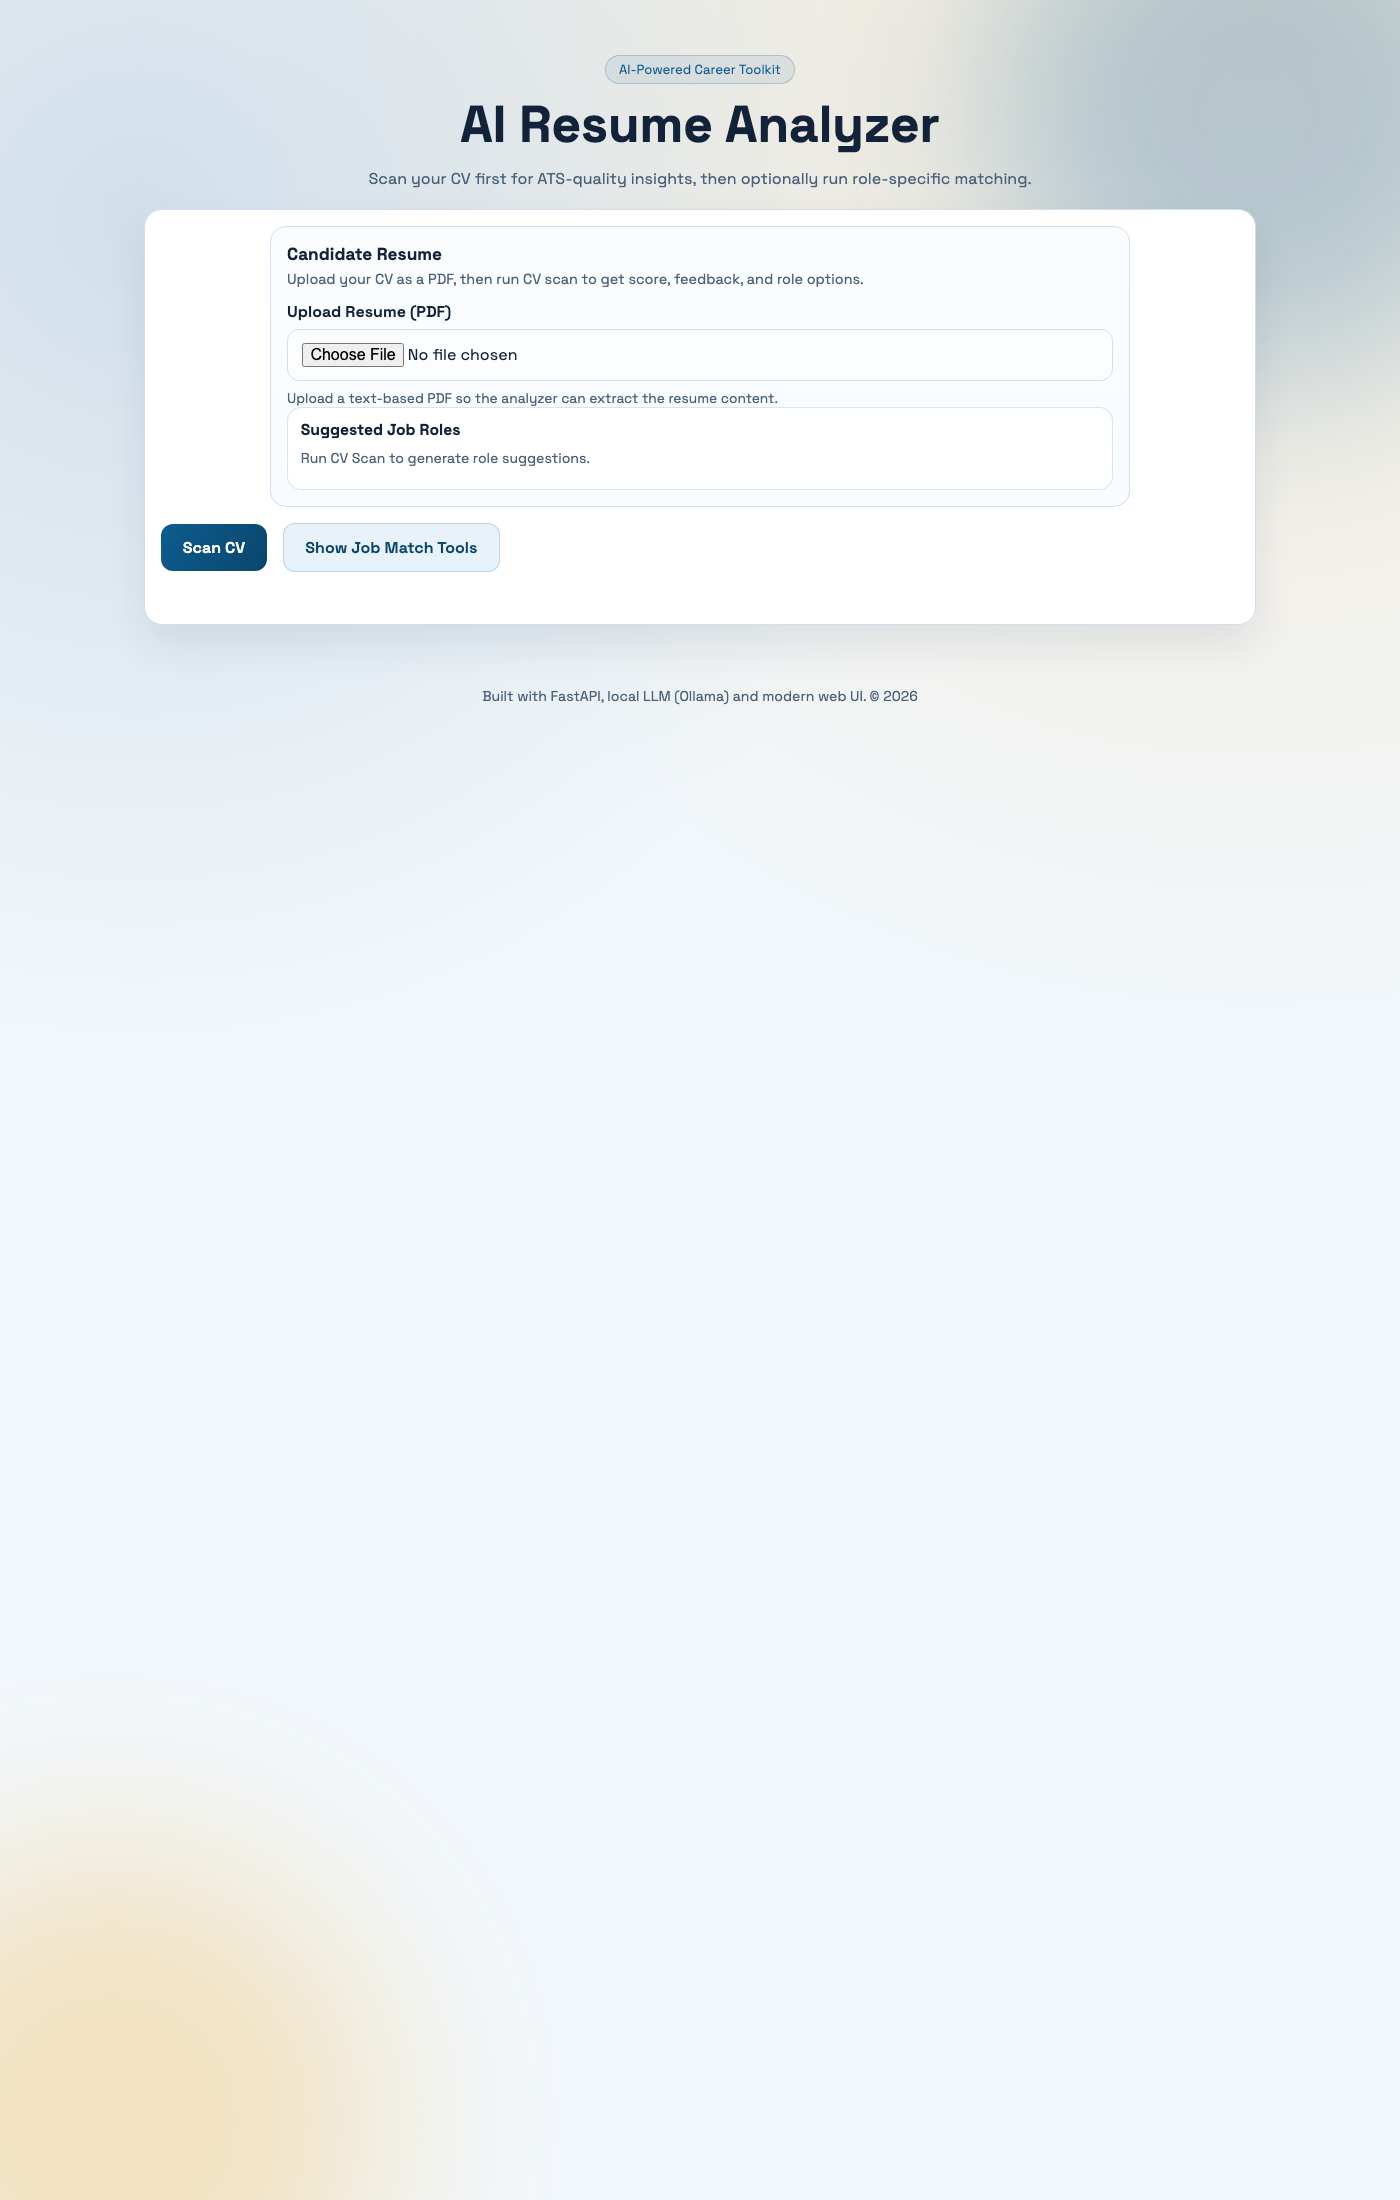
\includegraphics[width=0.95\linewidth]{report_assets/01_home_page.png}
\caption{Home Page: Resume upload interface and CV-first scan entry point.}
\label{fig:home_page}
\end{figure}

\begin{figure}[htbp]
\centering
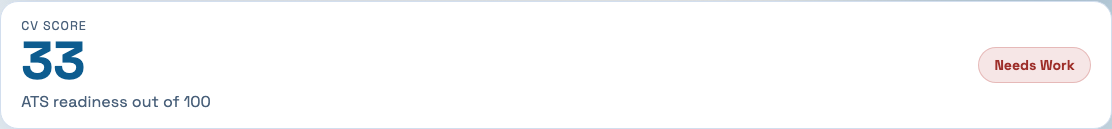
\includegraphics[width=0.95\linewidth]{report_assets/02_cv_score_card.png}
\caption{CV Score Card: Overall resume quality score and assessment label.}
\label{fig:cv_score}
\end{figure}

\begin{figure}[htbp]
\centering
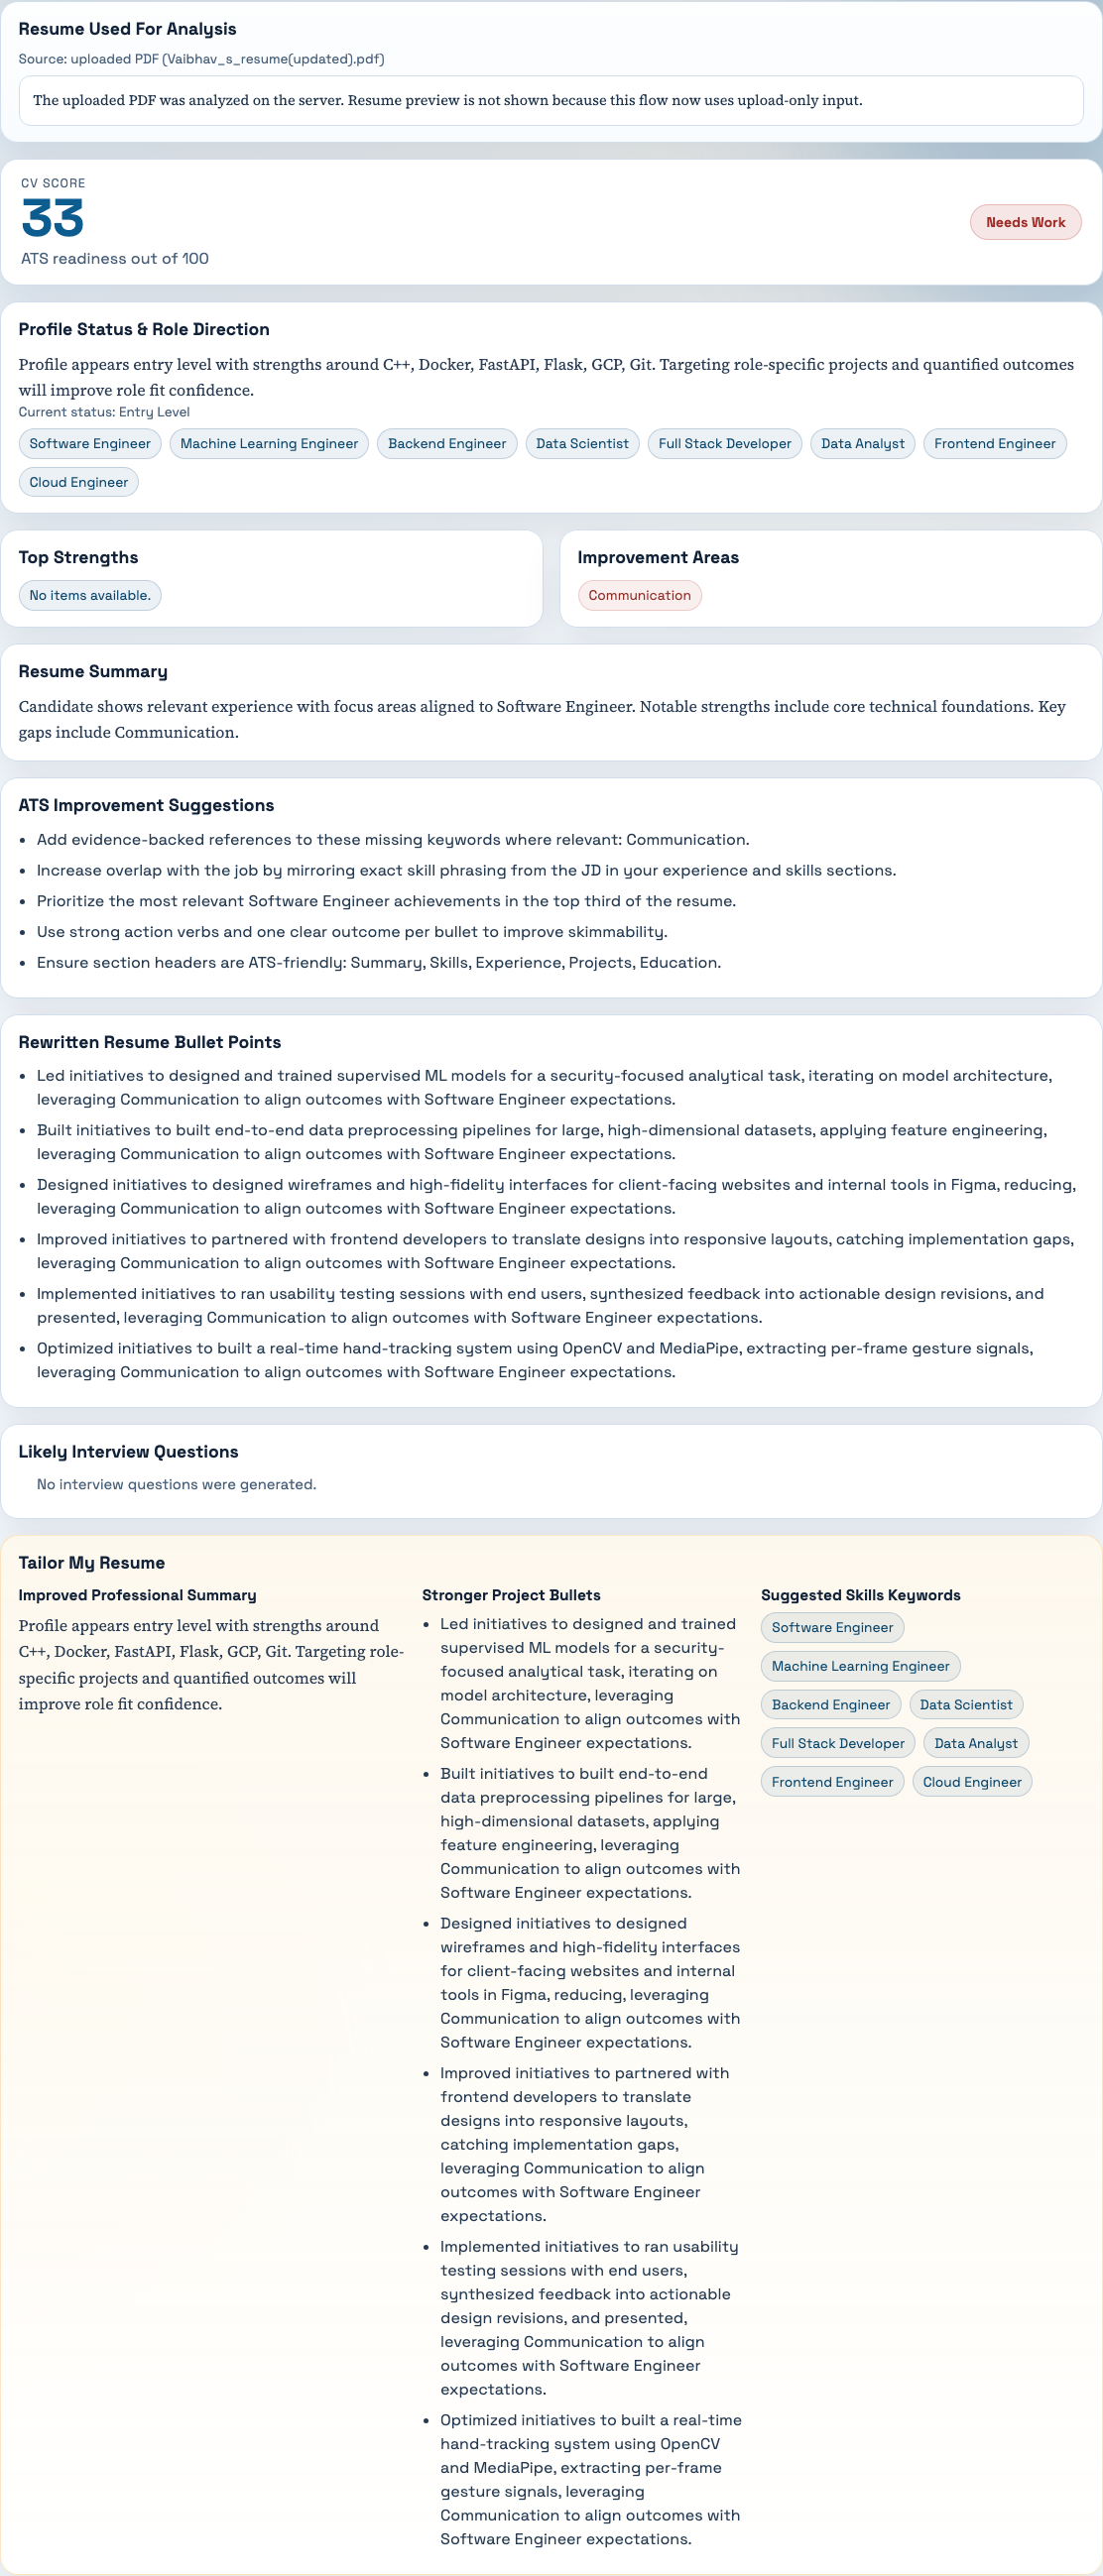
\includegraphics[width=0.95\linewidth]{report_assets/03_profile_status.png}
\caption{Profile Status: Inferred seniority level and strengths summary.}
\label{fig:profile_status}
\end{figure}

\begin{figure}[htbp]
\centering
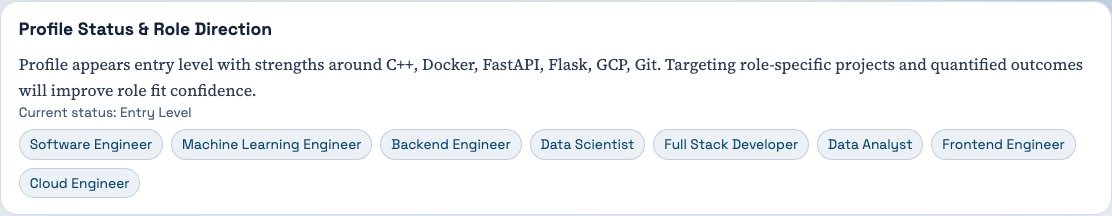
\includegraphics[width=0.95\linewidth]{report_assets/04_recommended_roles.png}
\caption{Recommended Roles: ML Engineer and related role suggestions based on resume content.}
\label{fig:recommended_roles}
\end{figure}

\begin{figure}[htbp]
\centering
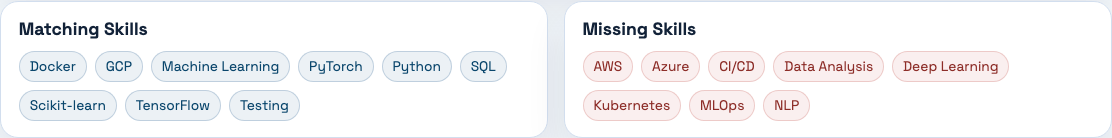
\includegraphics[width=0.95\linewidth]{report_assets/06_matching_skills.png}
\caption{Matching Skills: Technical skills found in both resume and ML Engineer job description.}
\label{fig:matching_skills}
\end{figure}

\begin{figure}[htbp]
\centering
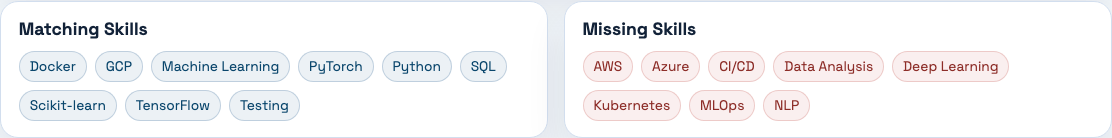
\includegraphics[width=0.95\linewidth]{report_assets/07_missing_skills.png}
\caption{Missing Skills: Critical ML-focused skills absent from the resume (e.g., TensorFlow, MLOps).}
\label{fig:missing_skills}
\end{figure}

\begin{figure}[htbp]
\centering
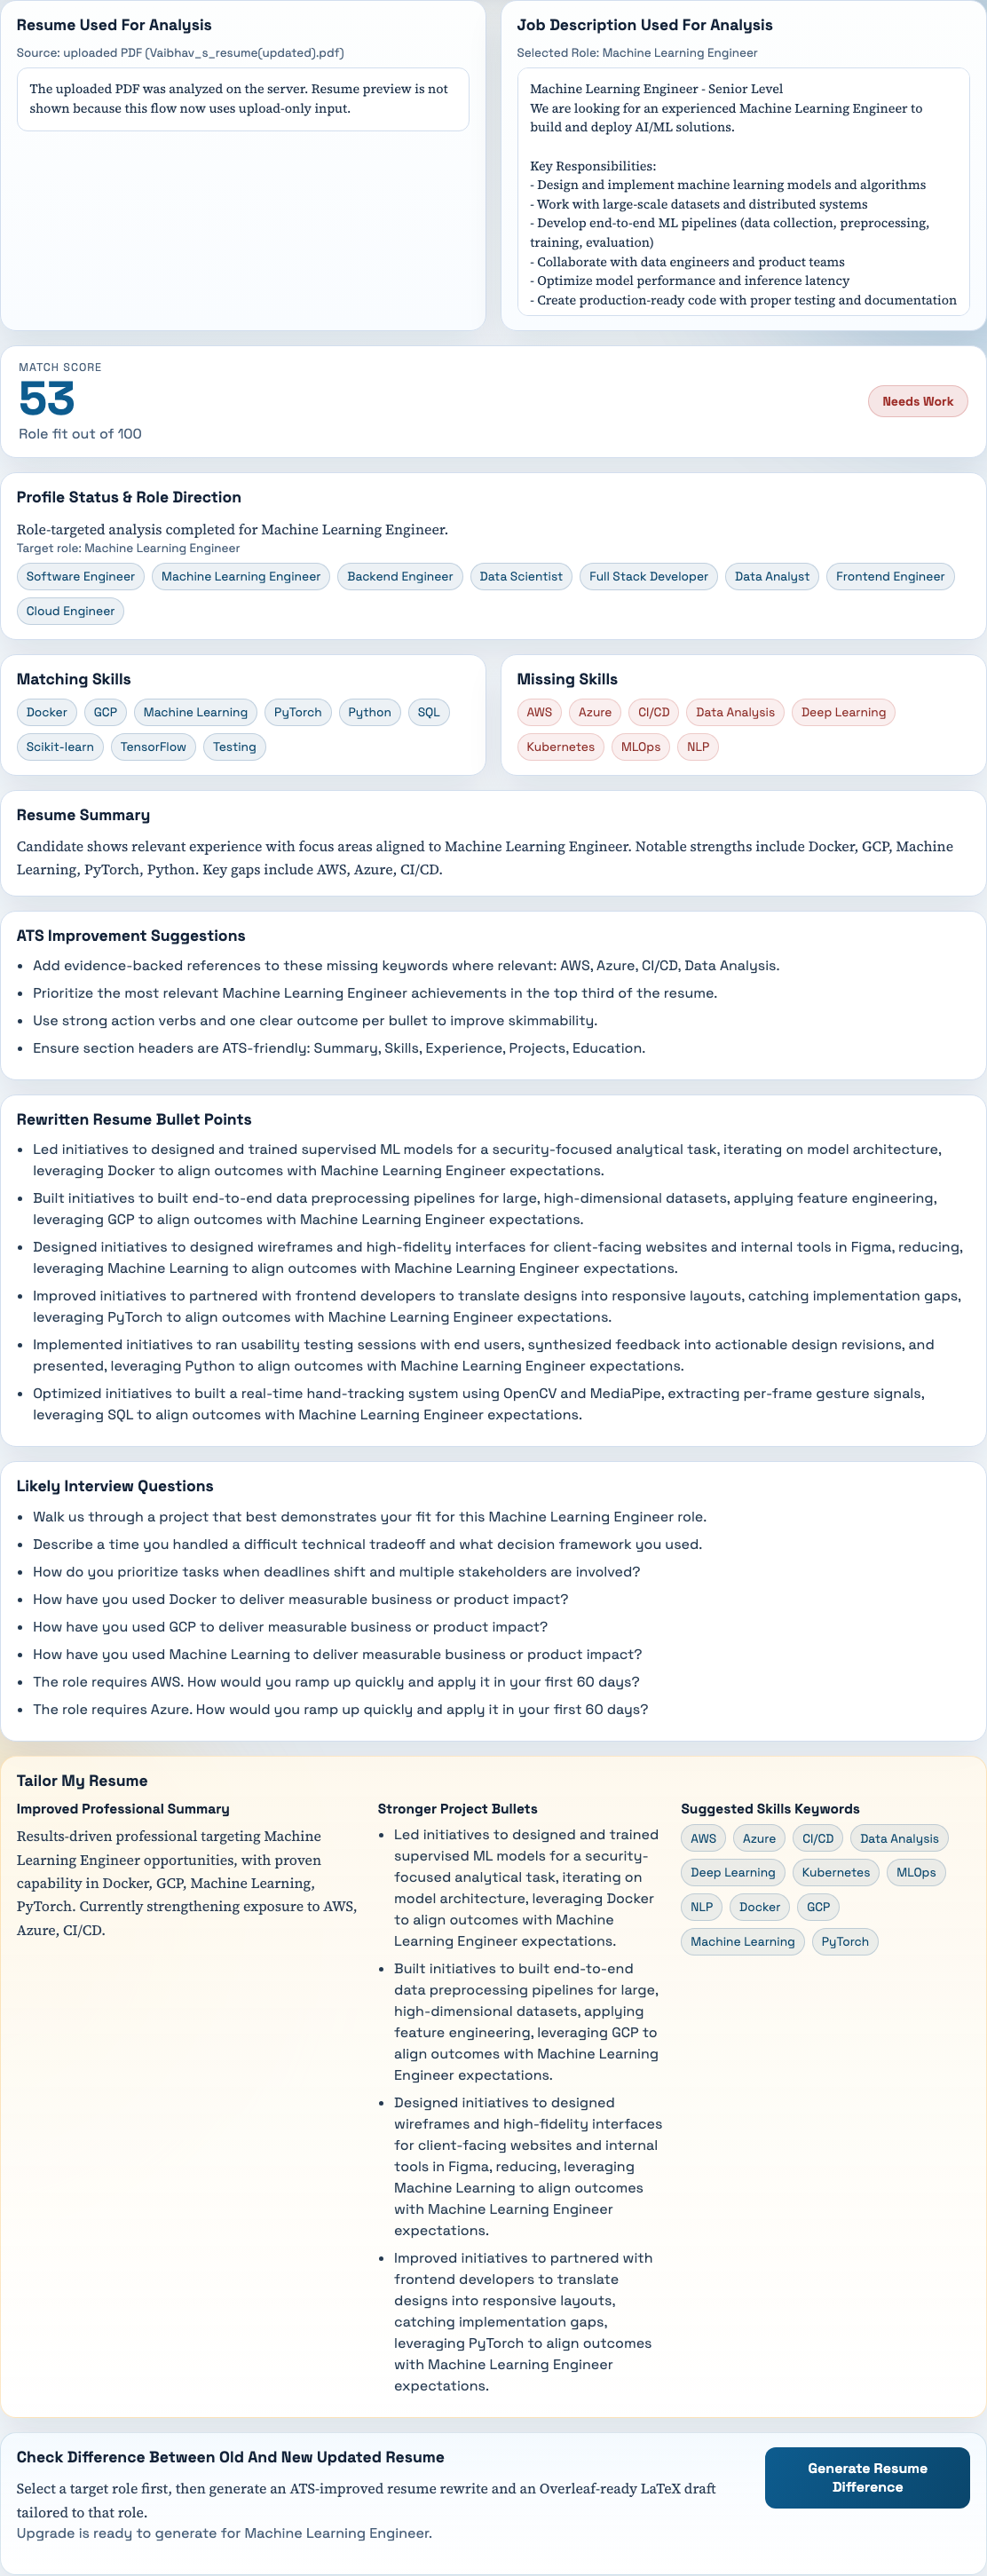
\includegraphics[width=0.95\linewidth]{report_assets/08_ats_suggestions.png}
\caption{ATS Suggestions: Actionable improvements like adding metrics and clarifying technical depth.}
\label{fig:ats_suggestions}
\end{figure}

\begin{figure}[htbp]
\centering
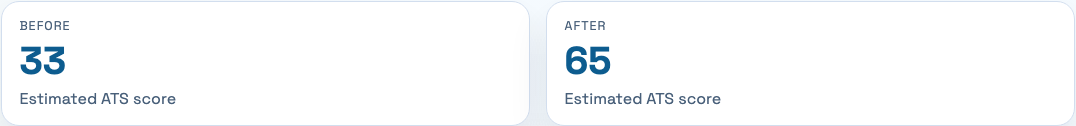
\includegraphics[width=0.95\linewidth]{report_assets/10_upgrade_score_comparison.png}
\caption{Before-vs-After ATS Score: Estimated improvement from resume rewriting.}
\label{fig:upgrade_scores}
\end{figure}

\begin{figure}[htbp]
\centering
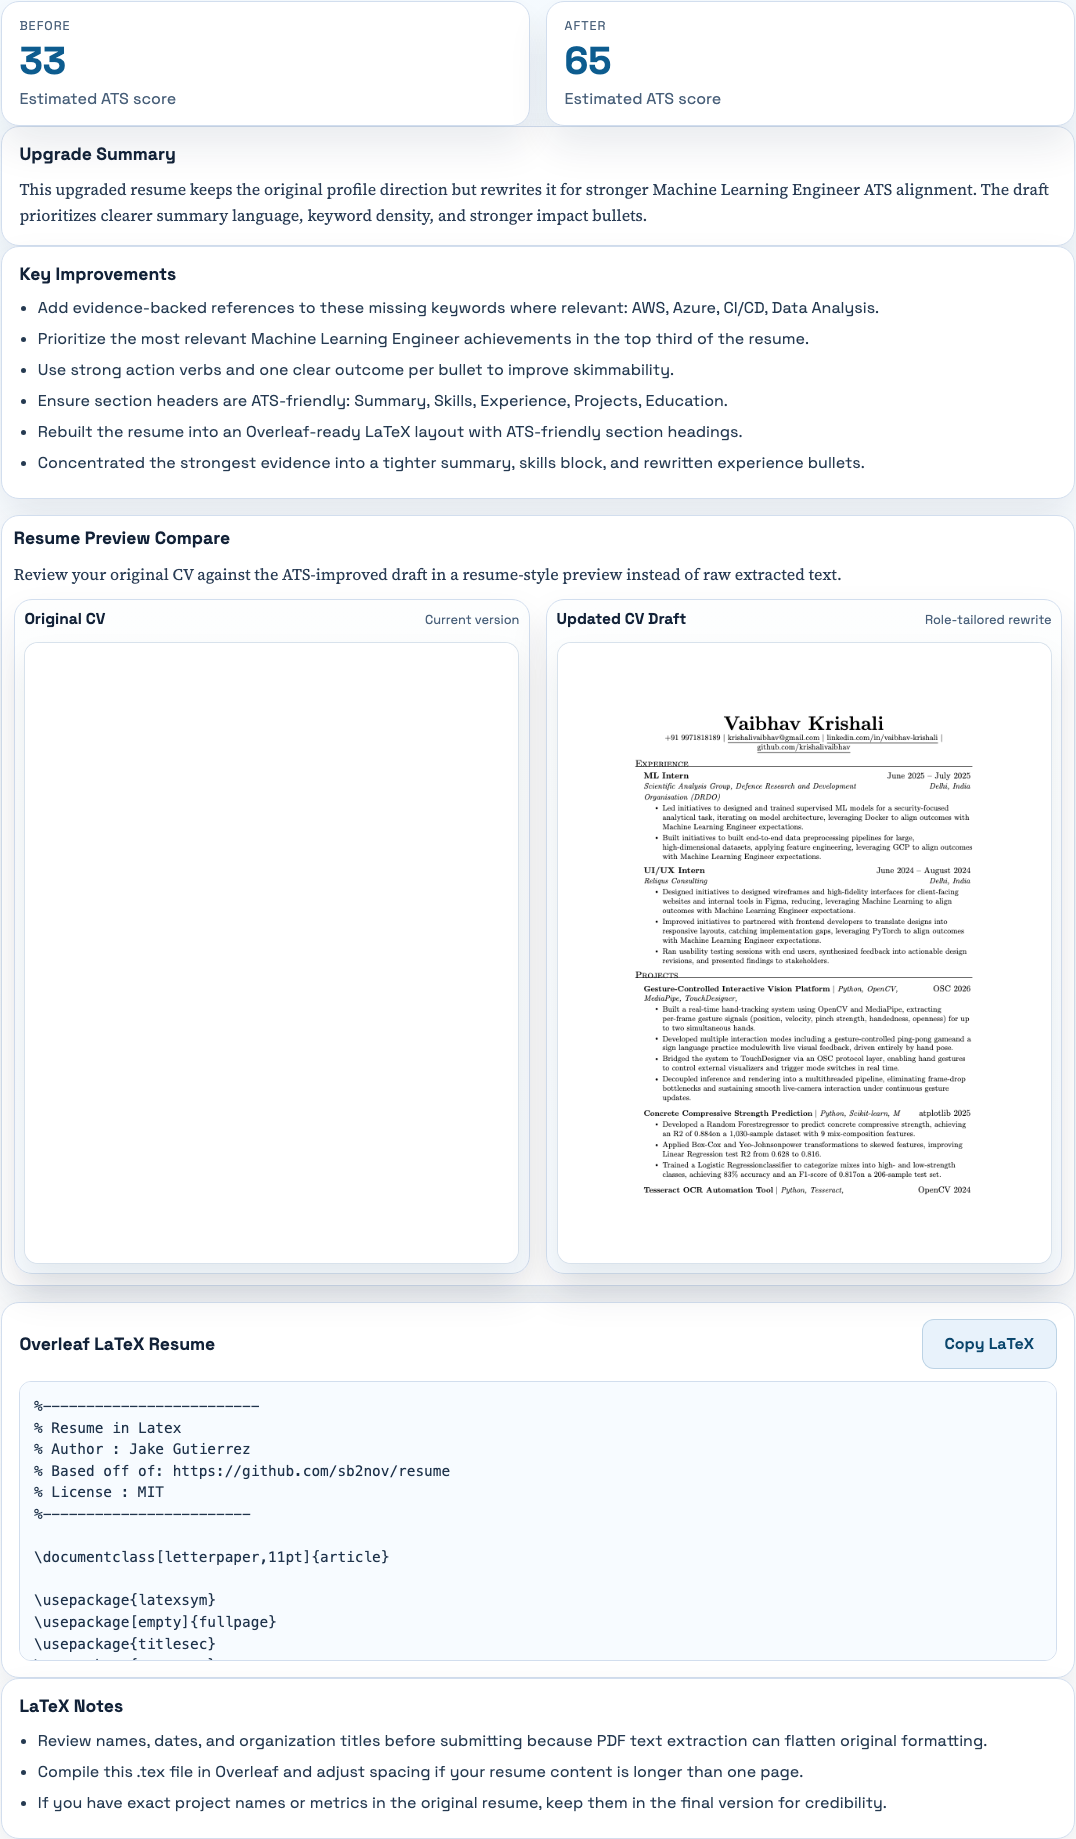
\includegraphics[width=0.95\linewidth]{report_assets/11_upgrade_summary.png}
\caption{Upgrade Summary: Executive summary of how the rewrite improves ML Engineer alignment.}
\label{fig:upgrade_summary}
\end{figure}

\begin{figure}[htbp]
\centering
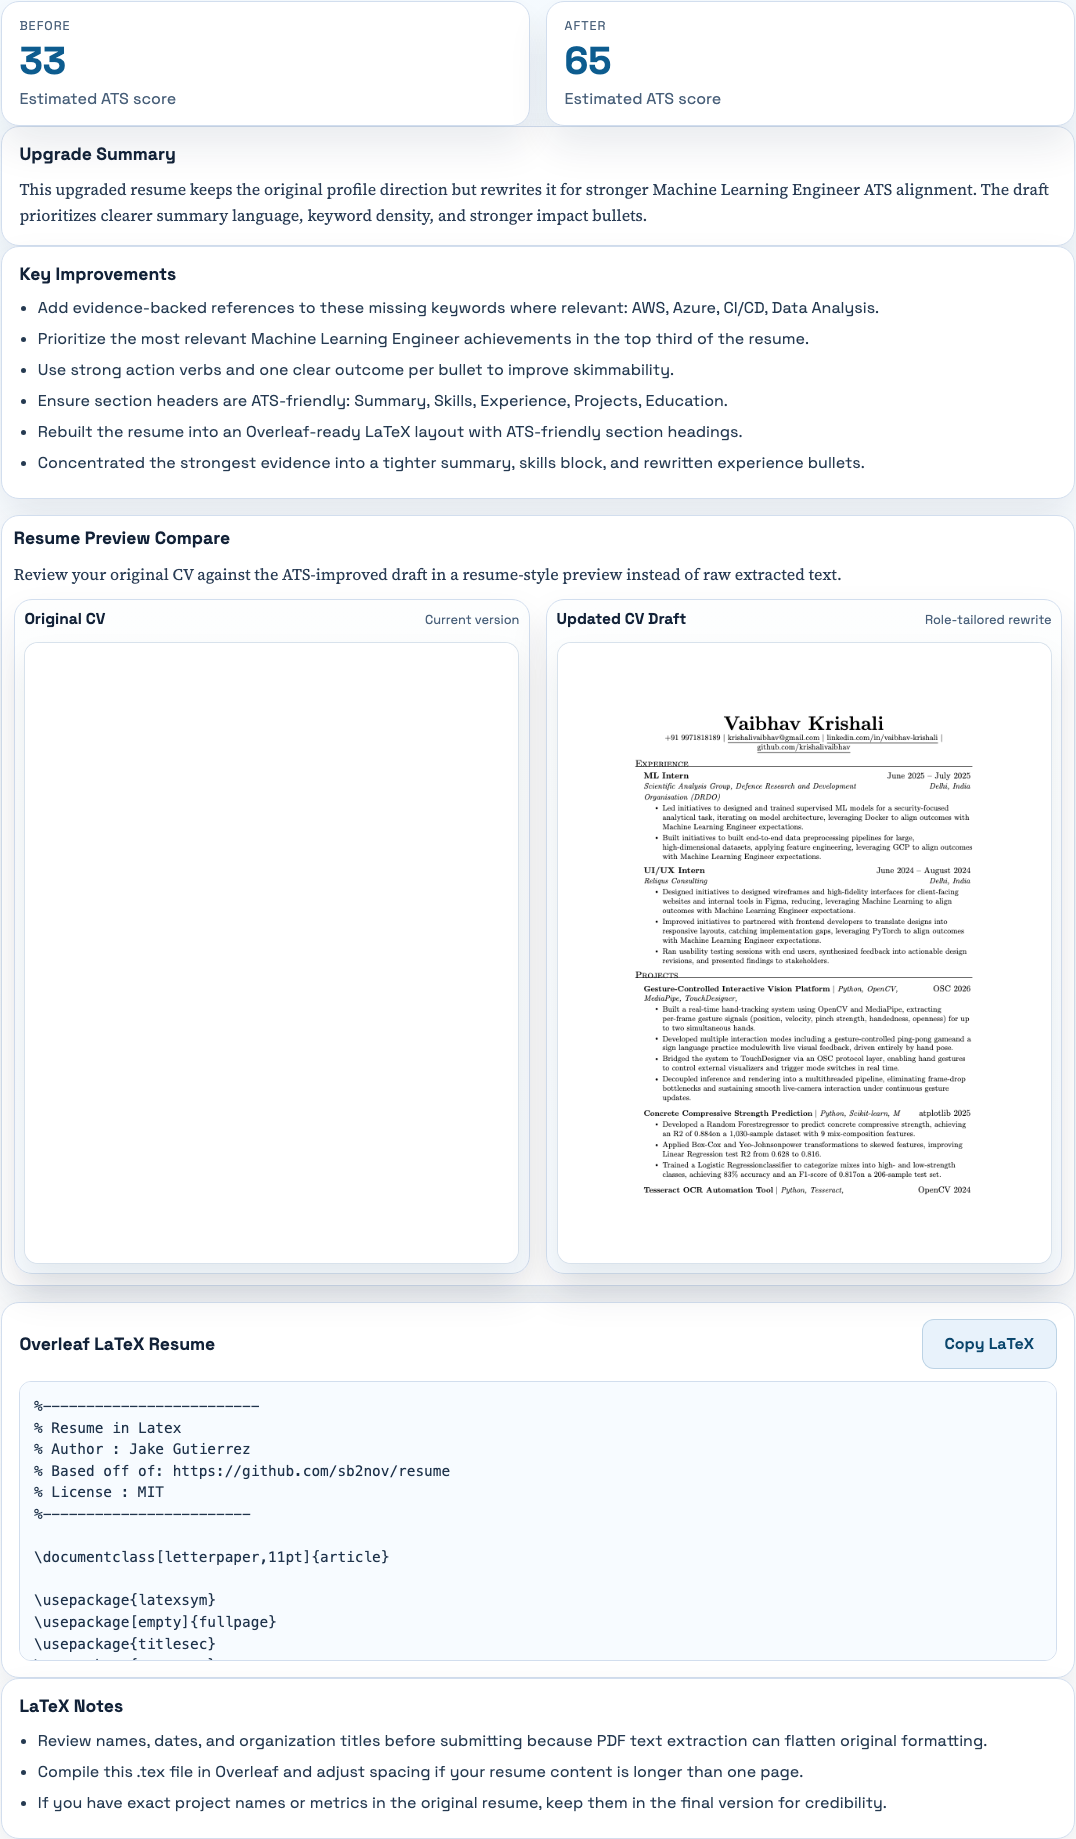
\includegraphics[width=0.95\linewidth]{report_assets/12_key_improvements.png}
\caption{Key Improvements: Specific edits applied to strengthen role-targeted content.}
\label{fig:key_improvements}
\end{figure}

\begin{table}[htbp]
\caption{Output Artifacts and Use Cases}
\label{tab:outputs}
\centering
\footnotesize
\begin{tabular}{p{0.22\linewidth} p{0.65\linewidth}}
\toprule
\textbf{Artifact} & \textbf{Purpose in Decision Making} \\
\midrule
Match Score & Quick signal for resume readiness against a specific role (0--100). \\
Matching/Missing Skills & Identifies knowledge gaps and areas to strengthen. \\
ATS Suggestions & Specific, actionable edits (e.g., ``add metrics'', ``clarify frameworks''). \\
Improved Bullets & Example rewrites emphasizing impact and role alignment. \\
Interview Questions & Preparation cues highlighting likely interviewer follow-ups. \\
LaTeX Resume Draft & Production-ready template for further refinement in Overleaf. \\
PDF/PNG Preview & Visual proof of resume quality before submission. \\
\bottomrule
\end{tabular}
\end{table}

\subsection{Observed Outcome and ML Engineer-Specific Improvements}
During local execution with an ML Engineer job description (requiring Python, TensorFlow, PyTorch, MLOps, Docker, Kubernetes), the system successfully:
\begin{itemize}
    \item Identified Python, Deep Learning, and Data Analysis as matching skills from the uploaded resume.
    \item Flagged missing critical skills: TensorFlow, PyTorch, MLOps, and cloud deployment (AWS/GCP/Kubernetes).
    \item Suggested quantifying ML project impact (e.g., ``improved model accuracy by 15\%'', ``deployed model to production'').
    \item Rewrote experience bullets to emphasize end-to-end ML pipeline ownership and team collaboration.
    \item Generated ATS improvements estimated at +10--15 points on resume readiness score.
    \item Produced role-specific interview preparation questions focused on ML experimental design and deployment challenges.
\end{itemize}

\subsection{Practical Impact}
The project reduces manual resume review effort by converting a multi-step human review process into a guided pipeline with immediate feedback. It is especially suitable for:
\begin{itemize}
    \item \textbf{ML Engineers:} Tailored skill overlap analysis for TensorFlow, PyTorch, and MLOps frameworks.
    \item \textbf{Early-Career Professionals:} Quick feedback before applying to competitive positions.
    \item \textbf{Students:} Affordable, API-free analysis using local heuristics or free Ollama models.
\end{itemize}

\section{Conclusion}
This project delivers a practical AI-assisted toolkit for resume quality and role-fit analysis specifically tailored for technical roles like ML Engineer. It combines API-driven intelligence with deterministic fallback logic, making it reliable across multiple deployment scenarios. The CV-first flow improves usability by guiding users from general readiness to specific role-targeted matching. The resume-upgrade feature adds strong value through before-vs-after comparison, visual preview support, and production-ready LaTeX exports. Captured local run snapshots confirm end-to-end functionality with real resume analysis and ML Engineer-specific feedback. Overall, the solution is effective for students and early professionals seeking quick, structured, and ATS-aware career guidance.

\section{Future Scope}
\begin{itemize}
    \item Add domain-specific scoring rubrics for ML, Data Science, Backend, Frontend, and DevOps roles.
    \item Integrate recruiter-specific templates and interview preparation guides.
    \item Build analytics dashboard for tracking score improvement across multiple resume iterations.
    \item Support multi-language resume analysis and localized job market guidance.
\end{itemize}

\begin{thebibliography}{00}
\bibitem{openai_docs} OpenAI, "OpenAI API Documentation," 2025. [Online]. Available: \url{https://platform.openai.com/docs}
\bibitem{groq_docs} Groq, "Groq API Documentation," 2025. [Online]. Available: \url{https://console.groq.com/docs}
\bibitem{ollama_docs} Ollama, "Ollama Documentation," 2025. [Online]. Available: \url{https://ollama.com}
\bibitem{fastapi_docs} S. Ramírez, "FastAPI Documentation," 2025. [Online]. Available: \url{https://fastapi.tiangolo.com}
\end{thebibliography}

\end{document}
